% This is samplepaper.tex, a sample chapter demonstrating the
% LLNCS macro package for Springer Computer Science proceedings;
% Version 2.20 of 2017/10/04
%
\documentclass[runningheads]{llncs}
%
\usepackage{xcolor}
\usepackage{graphicx}
\usepackage{makecell}
\usepackage{textcomp}
%\usepackage{amsmath,amssymb,amsfonts}
\usepackage{hyperref}
\usepackage{algorithm,algorithmic}
\usepackage{wrapfig}
\usepackage{mathtools}
\usepackage{tabularx}
\usepackage{etoolbox}

% Used for displaying a sample figure. If possible, figure files should
% be included in EPS format.
%
% If you use the hyperref package, please uncomment the following line
% to display URLs in blue roman font according to Springer's eBook style:
% \renewcommand\UrlFont{\color{blue}\rmfamily}

\renewcommand{\baselinestretch}{0.98}

\begin{document}
%
%\title{Automated Formal Synthesis of Optimal Sizing for Stand-alone Solar Photovoltaic Systems\thanks{Supported by Newton Fund (ref. 261881580) and FAPEAM (Amazonas State Foundation for Research Support, calls 009/2017 and PROTI Pesquisa 2018).}}
\title{Synthesis of Solar Photovoltaic Systems: Optimal Sizing Comparison\thanks{Supported by Newton Fund (ref. 261881580) and FAPEAM (Amazonas State Foundation for Research Support, calls 009/2017 and PROTI Pesquisa 2018).}}
%
%\titlerunning{Abbreviated paper title}
% If the paper title is too long for the running head, you can set
% an abbreviated paper title here
%
\author{Alessandro Trindade\inst{1} \and Lucas Cordeiro\inst{2}} %\orcidID{0000-0001-8262-2919} \orcidID{0000-0002-6235-4272}
%
\authorrunning{A. Trindade and L. Cordeiro}
% First names are abbreviated in the running head.
% If there are more than two authors, 'et al.' is used.
%
\institute{Federal University of Amazonas, Brazil, \email{alessandrotrindade@ufam.edu.br} \and
University of Manchester, UK, \email{lucas.cordeiro@manchester.ac.uk}}
\maketitle       % typeset the header of the contribution


\begin{abstract}
The use of power generation with renewable energy sources is proliferating due to industrial development. Photovoltaic (PV) panels have emerged as an alternative to the fossil or nuclear fuel energy generation. The use of formal methods for PV systems is a new subject with significant research spanning only the last five years. Here we develop and evaluate a sound, automated synthesis approach to obtain optimal sizing PV systems. We use a stand-alone configuration for this study since it is the most common system used for remote rural areas of developing countries or areas where the grid extension is infeasible. We propose a variant of the counterexample guided inductive synthesis (CEGIS) approach with two phases linking the technical and cost analysis. We advocate that the application of CEGIS to obtain optimal PV sizing has various advantages if compared to off-the-shelf optimization tools available in the market. Experimental results from seven case studies demonstrate that we can produce an optimal solution within an acceptable run-time; different software verifiers are evaluated to check performance and soundness. We also compare our CEGIS approach with a commercial tool specialized in PV systems optimization. Both results are validated with commercial design software; furthermore, some real PV systems comparison are used to show our approach effectiveness. 
\end{abstract}

%%%%%%%%%%%%%%%%%%%%%%%%%%%%%%%%%%%%%%%%%%%%%%%%%%%%%%%%
\section{Introduction}
%%%%%%%%%%%%%%%%%%%%%%%%%%%%%%%%%%%%%%%%%%%%%%%%%%%%%%%%
Lack of access to clean and affordable energy is considered a core dimension of poverty~\cite{Hussein2012}. Progress has been made worldwide; in particular, in 2017, the number of people without electricity access fell below $1$ billion thresholds for the first time~\cite{IEAweo2018}. The share of people without access to electricity from Africa is 58\%, while 19\% of the share comes from developing Asia, and 31\% from Latin America~\cite{IEAweo2018}. Numbers from Brazil show the aim to electrify 270 isolated areas and 2.7 million people by 2023~\cite{EPE2018}. 
There exists a close relationship between the lack of energy and the low HDI (Human Development Index) of those localities~\cite{Coelho}. It follows that increased access to energy allows economic growth and poverty alleviation \cite{Karekesi}. In order to provide electricity for all, decentralized systems led by solar photovoltaic (PV) in off-grid and mini-grid systems will be the lowest-cost solution for three-quarters of the connections needed~\cite{Hussein2012}. 

In order to evaluate a PV system, there exist various specialized tools, e.g., RETScreen~\cite{Pradhan} and HOMER~\cite{Swarnkar}; and even general-purpose tools, e.g., MATLAB/Simulink~\cite{Gow1999}. However, these tools are based on simulation; they have the drawback of an incomplete coverage since verification of all possible combinations, and potential failures of a system are infeasible~\cite{ClarkeHV18}. Non-linear optimization tools could be employed since a PV system is typically modeled as a non-linear set of equations. However, the industry demands the final solution to be the optimum, considering manufacturers, models, and brands available on the market and not just minimum or maximum powers and values for the optimized items, which can only be achieved with specialist PV optimization software.

Optimization of PV systems is not a recent topic; since the 1990s, different techniques using different criteria to find ultimate combinations for design parameters, based on intuitive, numerical, and analytical methods, were proposed and developed~\cite{Alsadi2018}. In $2015$, an automated simulation-based verification technique was applied to verify the correctness of power system protection settings~\cite{Sengupta2015}. In $2017$, a researcher suggested the application of formal methods to verify and control the behavior of computational devices in a smart grid ~\cite{Abate2017}. In $2018$, a verification methodology was applied to PV panels and its distributed power point tracking~\cite{Driouich2018}. In $2019$, an automated verification methodology was proposed to validate stand-alone solar PV systems~\cite{TrindadeCordeiro19}. However, \textit{formal methods and its application to synthesize PV systems are still unexplored in literature}.

Here we developed a variant of the counterexample guided inductive synthesis (CEGIS)~\cite{DBLP:conf/asplos/Solar-LezamaTBSS06} technique for synthesizing optimal sizing of stand-alone PV systems using commercial equipment data. Given a correctness specification $\sigma$, our method uses that as a starting point and then iteratively produces a sequence of candidate solutions that satisfy $\sigma$, related to power reliability. In particular, on each iteration, we synthesize the sizing of stand-alone PV systems, but that may not achieve the lowest cost. The candidate solution is then verified via model checking with a lower bound that serves as the minimum cost of reference. If the verification step does not produce a counterexample, then the lower bound is adjusted; otherwise, we have achieved an optimal PV sizing.

Our work makes three significant contributions to advance the state-of-the-art in PV optimal sizing. First, the use of automated verification in PV systems was uncommon in recent prior studies; we have shown that formal methods can detect various errors in PV systems designed by existing commercial tools~\cite{TrindadeCordeiro19}. Here the application of formal methods to synthesize PV sizing is novel, thereby leading to more accurate results than existing commercial tools. Second, we evaluate our approach using different state-of-the-art verifiers to obtain the best performance in our verification back-end for synthesizing optimal PV systems. We compare that to HOMER Pro optimization, with the results being validated with accurate commercial design software called PVsyst. Lastly, we discuss the challenges of applying formal methods to PV systems and reflect on lessons learned from this experience.

\vspace{-2ex}

%-----------------------------------------------------------
\section{Preliminaries}
\label{sec:AutomatedVerification}
%-----------------------------------------------------------
\vspace{-1ex}

Fig.~\ref{fig:optimization} illustrates how to obtain the optimal sizing of a stand-alone PV system using the traditional techniques (manual and simulation) and the proposed synthesis technique. Note that the input information is the same for all the methods: weather data, price information, design requirements, as load curve and power demand, and design assumptions. For the automated synthesis, we also define the bound $k$ to restrict the design-space search. Here we start with a low bound $k$ and incrementally increase it to avoid time and memory constraints on our verification back-end. Therefore, the proper choice of $k$ is essential to this method.

\begin{figure}[h]
\fbox{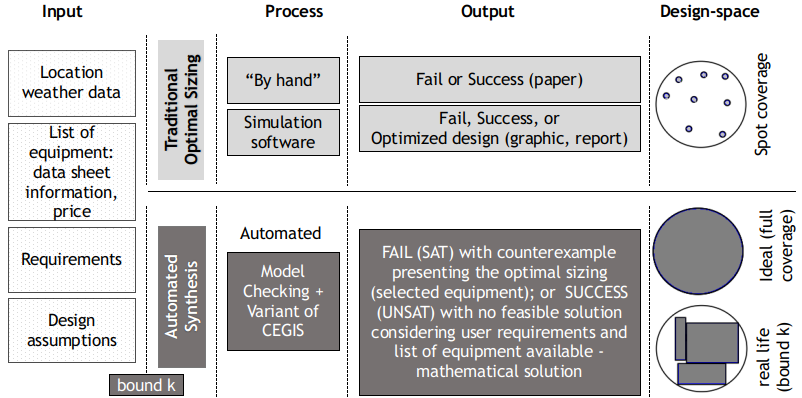
\includegraphics[width=0.9\textwidth]{optimalsizingprocess4}}
\centering
\caption{Comparison of optimal sizing methods.}
\label{fig:optimization}
\end{figure}

Both techniques (traditional and automated synthesis) produce as output either a SUCCESS or FAIL result, thereby considering a feasible technical solution with the lowest cost. On the one hand, when done by simulation, we get a report or graphical result; on the other hand, the automated synthesis technique, which is mathematical reasoning of a model, presents a counterexample with the optimal solution stored in variables. Furthermore, the design-space coverage during the optimal sizing search is sound and complete when using synthesis.

%-----------------------------------------------------------
\subsection{Program Synthesis}
\label{sec:ProgramSynthesis}
%-----------------------------------------------------------
The basic idea of program synthesis is to automatically construct a program $P$ that satisfies a correctness specification $\sigma$. In particular, program synthesis is automatically performed by engines that use a correctness specification $\sigma$, as a starting point, and then incrementally produce a sequence of candidate solutions that partially satisfy $\sigma$~\cite{Abateetal2017}. As a result, a given candidate program $p$ is iteratively refined to match $\sigma$ more closely. Figure~\ref{Counter-Example-Guided-Inductive-Synthesis} illustrates the underlying architecture. 

\begin{figure}[h]
\begin{center}
\fbox{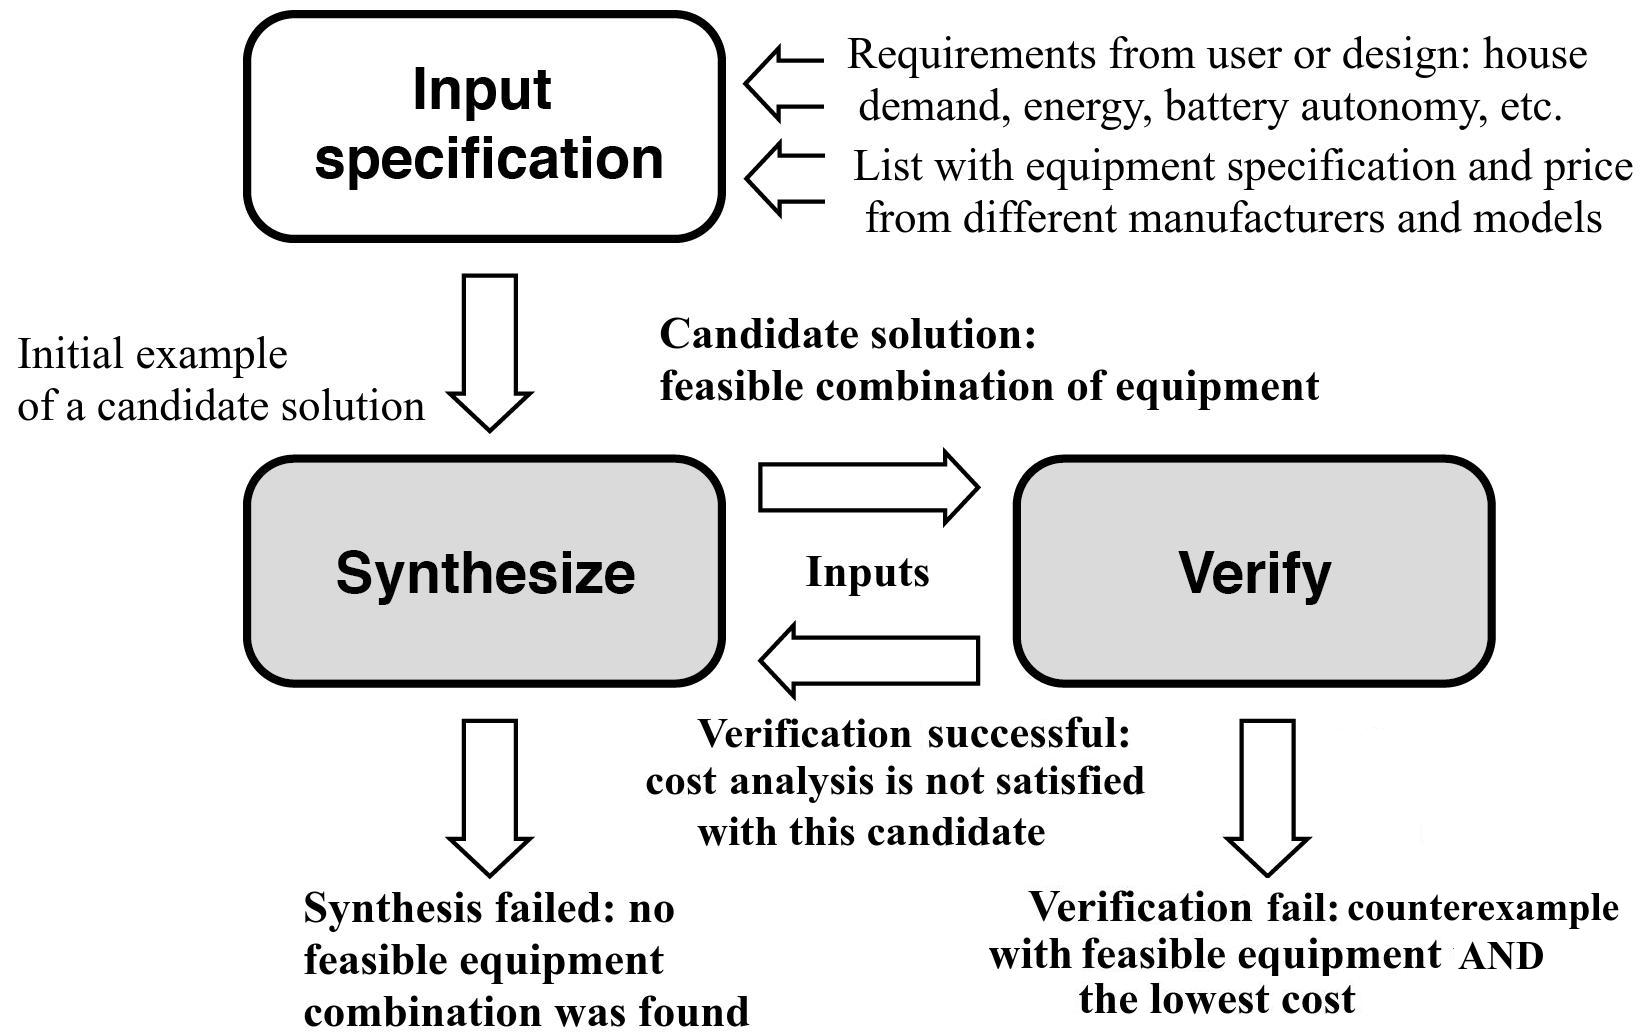
\includegraphics[width=0.75\textwidth]{fig2_rev2.jpg}}
\end{center}
%
%\begin{wrapfigure}{r}{0.5\textwidth}
%\begin{center}
%	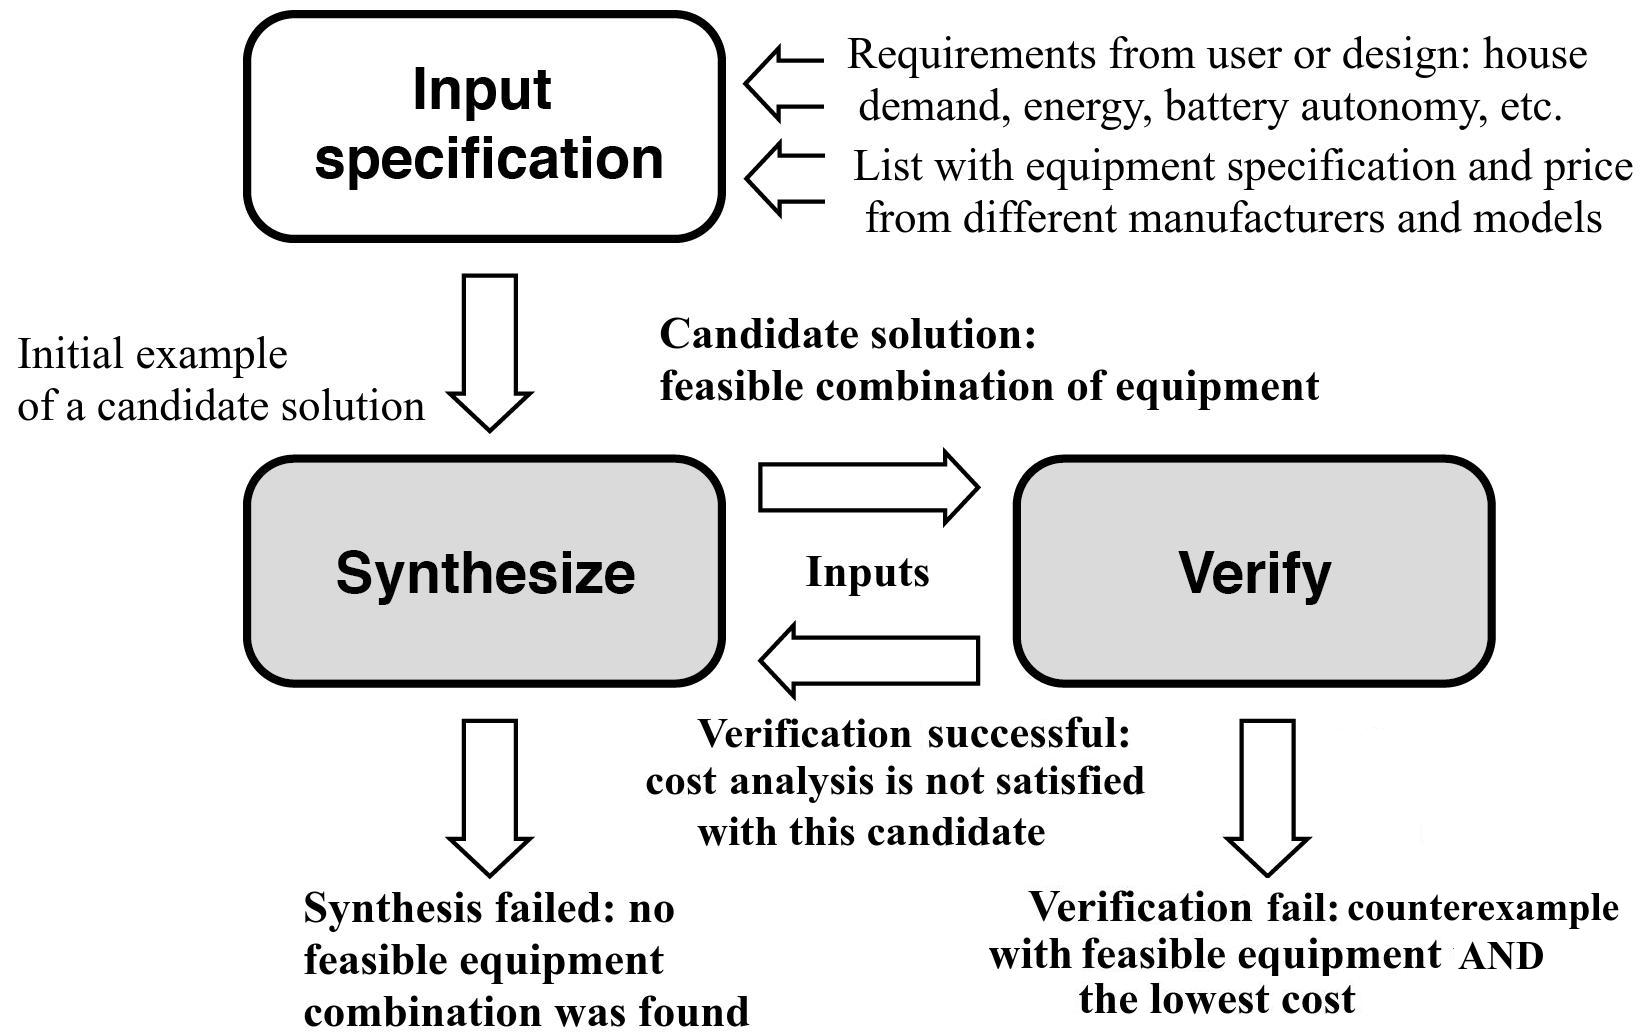
\includegraphics[width=0.5\columnwidth]{fig2_rev2.jpg}
%\end{center}	
	\caption{CEGIS in PV system sizing.}
	\label{Counter-Example-Guided-Inductive-Synthesis}
%\end{wrapfigure}
\end{figure}

The correctness specification $\sigma$ provided to our synthesizer is of the form $\exists \vec{F}. \forall \vec{x}. \sigma(\vec{x}, \vec{F})$, where $\vec{F}$ ranges over functions, $\vec{x}$ ranges over ground terms, and $\sigma$ is a quantifier-free (QF) formula typically supported by SMT solvers. The ground terms are interpreted over some finite domain $\mathcal{D}$, where $\mathcal{D}$ can be encoded using the SMT's bit-vectors part. Our specification includes house demand, energy, and battery autonomy; we also provide equipment specifications and prices from different manufacturers and models.

In Figure~\ref{Counter-Example-Guided-Inductive-Synthesis}, the phases {\sc Synthesize} and {\sc Verify} interact via a finite set of test vectors {\sc inputs}, which is incrementally updated. Given the correctness specification $\sigma$, the {\sc Synthesize} procedure tries to find an existential witness $\vec{F}$ satisfying the specification $\sigma(\vec{x}, \vec{F})$, for all $\vec{x}$ in {\sc inputs} (as opposed to all $\vec{x} \in \mathcal{D}$). If {\sc Synthesize} succeeds in finding a witness~$\vec{F}$, the latter is a candidate solution to the full synthesis formula, which is passed to {\sc Verify} to check whether it is a proper solution ({\it i.e.}, $\vec{F}$ satisfies the specification $\sigma(\vec{x}, \vec{F})$ for all $\vec{x}\in\mathcal{D}$). If this is the case, then the algorithm terminates.

One may notice that each iteration of the traditional CEGIS loop adds a new input to the finite set $INPUTS$, which is then used for synthesis. Given that the full set of inputs $\mathcal{D}$ is finite because we use bit-vector expressions, this means that the refinement loop can only iterate over a finite number of times. However, {\sc Synthesize} may conclude that no candidate solution obeying $\sigma$ for the finite set $INPUTS$ exists. 

In our CEGIS variant, there exist four differences related to the traditional one: 
(1) there exists no test vector and every candidate is generated in the {\sc Synthesize} phase and sent to the {\sc Verify} phase; 
(2) if the {\sc Verify} phase is unsuccessful, then a new candidate is generated by {\sc Synthesize} and 
(3) the lower bound of the {\sc Verify} phase is incremented to search for the lowest cost; as a result,
(4) there exists no refinement from the {\sc Verify} phase back to the {\sc Synthesize} phase. In particular, a new counterexample is not added to the {\sc input} set since a failure during the {\sc Verify} phase will only discard a given candidate, which could be feasible in the next iteration with a new lower bound.

%%%%%%%%%%%%%%%%%%%%%%%%%%%%%%%%%%%%%%%%%%%%%%%%%%%%%%%%
\subsection{Sizing Stand-alone Solar PV Systems}
\label{sec:sizing}
%%%%%%%%%%%%%%%%%%%%%%%%%%%%%%%%%%%%%%%%%%%%%%%%%%%%%%%%

A PV system is illustrated in Fig.\ref{fig:blockdiagram}. It 
employs: the PV generator, which can be a \textbf{panel or an array}, is a semiconductor device that can convert solar energy into DC electricity; for night hours or rainy days, we hold \textbf{batteries} where power can be stored and used; the use of batteries as a storage form implies the presence of a \textbf{charge controller}~\cite{Hansen}; the PV arrays produce DC, and therefore when the PV system contains an AC load, a DC/AC conversion is required (\textbf{inverter}); the \textbf{AC load} dictates the behaviour of the AC electrical load from the house that will be fed by the system.

\begin{figure}[h]
\fbox{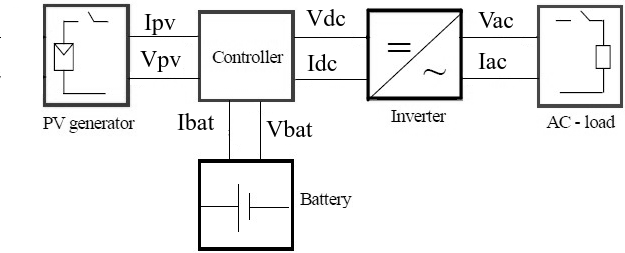
\includegraphics[width=0.8\textwidth]{blockdiagramPVS2_rev}}
\centering
\caption{Block diagram for a typical stand-alone PV system~\cite{Hansen}.}
\label{fig:blockdiagram} 
\end{figure}

The sizing check stage can ensure that the system meets the standard project steps related to the critical period method (worst month) for solar energy system sizing~\cite{Pinho} and adopting an MPPT (Maximum Power Point Tracking) charge controller, which is the most common in use. Firstly, we need to correct the daily energy consumption estimated for the load ($E_{consumption}$), which is carried out by Eq.~\eqref{eq:Ecorrected}, where the efficiency of batteries ($\eta_{b}$), controller ($\eta_{c}$), and inverter ($\eta_{i}$) are considered~\cite{Pinho} as follows

\begin{equation}
\label{eq:Ecorrected}
E_{corrected} = \dfrac{E_{consumption}}{\eta_{b} \times \eta_{c} \times \eta_{i} }.
\end{equation}

We must estimate the total power that will be demanded from the PV panels, as defined by Eq. ~\eqref{eq:Pminpanel}.

\begin{equation}
\label{eq:Pminpanel}
P_{min,panels} = \dfrac{1.25 \times E_{corrected}}{Insolation},
\end{equation}

\noindent where $Insolation$, also called solar irradiation or solar exposure, is expressed in terms of $kWh/m^{2}$ per day and depends on the site where the PV system will be deployed. A factor of $20$\% for losses is considered, because $1.25 = 1 \mathbin{/} (1 - 0.2)$.

On the one hand, the sizing must meet this requirement of minimum power supplied from the PV panels $P_{min,panels}$. On the other hand, the arrangement, if in series or parallel connections, it will depend on the charge controller specification of current $I_{c}$ and voltage $V_{c}$, as shown in Eq.~\eqref{eq:Icmin} and 
\eqref{eq:Vcmin}.

\begin{subequations}
 \begin{tabularx}{\textwidth}{Xp{1cm}X}
\begin{equation}
\label{eq:Icmin}
I_{c} \geq I_{total,PVpanels},
\end{equation}
 & &
\begin{equation}
\label{eq:Vcmin}
V_{c} \geq V_{total,PVpanels},
\end{equation}
\end{tabularx}
\end{subequations}

Related to the batteries, the energy $E_{b}$ to be demanded by the PV system, in order to meet the load requirements, is defined by Eq.~\eqref{eq:Ebat}.

\begin{equation}
\label{eq:Ebat}
E_{b} = \dfrac{Autonomy \times E_{corrected}}{DOD},
\end{equation}

\noindent where $Autonomy$ is the number of days expected for the PV system to work even when rain or clouds avoid the recharging of batteries usually is a design definition and has a value ranging from $0.5$ to $2$ days. $DOD$ is the depth of discharge or the fraction of discharge. The $DOD$ is usually $25$\% for lead-acid batteries, and $80$\% for lithium batteries; that represents a State of Charge ($SOC$) of $75$\% and $20$\% respectively, because $SOC=1-DOD$. However, it is worth separating the $DOD$ into two different definitions when the battery autonomy is bigger than one day ($24$ hours). Therefore, here in this thesis, the definition given here is for a maximum of $DOD$. When we deal with daily $DOD$, we will call it $DOD_{day}$, and obviously, the sum of every $DOD_{day}$ can not exceed the maximum $DOD$.

In order to define the $DOD_{day}$ we use Eq.~\eqref{eq:DODday}. Moreover, the minimum current from the DC bus is defined by Eq.~\eqref{eq:Idcbus}. This equation is important to define the battery arrangement of the system (series and parallel connections).

\begin{subequations}
 \begin{tabularx}{\textwidth}{Xp{1cm}X}
\begin{equation}
\label{eq:DODday}
DOD_{day} = \dfrac{E_{corrected} \times 100}{E_{b}},
\end{equation}
 & &
\begin{equation}
\label{eq:Idcbus}
I_{min,DCbus} = \dfrac{E_{b}}{V_{system}},
\end{equation}
\end{tabularx}
\end{subequations}

\noindent where $V_{system}$ is the DC voltage of the bus. 

As for batteries, we must first define the total capacity of the battery bank, which can be described as

\begin{equation}
\label{eq:Cbank}
C_{bank} = \dfrac{Autonomy E_{load}}{DOD \eta _{b} V_{system}},
\end{equation}

\noindent where $ E_{load} $ is the average energy consumed by the load corrected according to PV equipment efficiency, and $ \eta_{b} $ is the efficiency of the battery.

Equation \ref{eq:batcheck} then performs the final sizing check, considering the number of batteries in series ($ N_{BS} $) and the number of batteries in parallel ($ N_{BP} $) adopted in the project.

\begin{equation}
\label{eq:batcheck}
\left( N_{BS} \times N_{BP} \right) \geq N_{B}total
\end{equation}

The charge controller must initially meet the voltage requirement of the PV system, as described by Eq.~\eqref{eq:vcvsystem}.
 
\begin{equation}
\label{eq:vcvsystem}
V_{c} = V_{system}.
\end{equation}

The short circuit reference information from the manufacturer's solar panel must be corrected to the cell temperature because field temperature is higher than nominal or laboratory temperature, and the PV system is temperature dependent, as shown by Equation~\eqref{eq:iscamb}. 

\begin{equation}
\label{eq:iscamb}
I_{sc,amb} = \dfrac{G}{G_{ref}} \left[ I_{sc,ref} + \mu_{I} \times (T-25) \right]. 
\end{equation}

The controller must meet the maximum current from the PV array given by Eqs.~\eqref{eq:icmin} and~\eqref{eq:icicmin}.

\begin{subequations}
 \begin{tabularx}{\textwidth}{Xp{1cm}X}
\begin{equation}
\label{eq:icmin}
I_{c,min} = I_{sc,amb} \times N_{PP},
\end{equation}
& &
\begin{equation}
\label{eq:icicmin}
I_{c} \geq I_{c,min}.
\end{equation}
\end{tabularx}
\end{subequations}

The number of controllers required for the off-grid PV system, as defined by \cite{Yatimi}, is calculated using Equation \ref{eq:numberofcmin}. Besides, the final sizing check is performed by Equation \ref{eq:numberofc}, which validates the number of controllers adopted.

\begin{equation}
\label{eq:numberofcmin}
number_{controllers} = \dfrac{Total \, max \, power \, of \, PV}{Controller \, max \, power} = \dfrac{P_{m,ref} \times N_{TP}}{V_{system} \times I_{controller,max}}
\end{equation}

\begin{equation}
\label{eq:numberofc}
N_{controller} \geq number_{controllers}
\end{equation}

The inverter sizing check is performed through three equations. Eq.~\eqref{eq:vindc} ensures that the input voltage of the controller meets the system voltage. Eq.~\eqref{eq:voutac} ensures that the output voltage of the controller meets the AC voltage of the load, i.e., the outlet voltage. Finally, Eq.~\eqref{eq:invcheck} ensures that the controller can support the total demand of the load ($Demand$) and the surge power ($P_{surge}$), where $V_{in}DC$ is the nominal input voltage, and $V_{out}AC$ is the nominal output voltage of the inverter; $MAX_{AC,ref}$ is the peak power that the inverter can support.

\begin{subequations}
 \begin{tabularx}{\textwidth}{Xp{1cm}X}
\begin{equation}
\label{eq:vindc} 
V_{in}DC = V_{system}.
\end{equation}
& &
\begin{equation}
\label{eq:voutac} 
V_{out}AC = V_{AC}.
\end{equation}
\end{tabularx}
\end{subequations}

\begin{equation}
\label{eq:invcheck} 
\left[ (Demand \leq P_{AC,ref}) \, and \, (P_{surge} \leq MAX_{AC,ref}) \right].
\end{equation}

Some inverter models allow parallel operation of more than one unit, besides the integration in order to create bi-phase and three-phase circuits. It is advisable to use pure sine wave inverters, especially for electronic loads sensitive to harmonic distortion waves.

Besides that, it is crucial to verify the compatibility between the charge controller and inverter because some models are not compatible with equipment from other manufacturers. Furthermore, it is vital to select an inverter power that is lower than (or equal) the charge controller power, because the demand from the electric load causes the inverter to transfer this demand from the DC side. Then the controller can be overcharged during this operation and to burn.

All the equations above model the continuous-time behavior of the PV system; they produce real numbers except for the batteries and panels, where real numbers must be converted into integer ones, considering the minimum or maximum according to each equation. The verification and simulation tools need to handle non-linear real arithmetic to produce the correct result.

%------------------------------------------------------
\section{Synthesizing Optimal Sizing of Stand-alone Solar Photovoltaic Systems}
%------------------------------------------------------

The optimal sizing of PV systems is made by the best compromise between two objectives: \textit{power reliability} and \textit{system cost}~\cite{Alsadi2018}. This study will rely on the critical period solar energy method~\cite{Pinho}, as described in Section~\ref{sec:sizing}. Based on the fact that the deployment location is not specified, our study will use an adapted Life Cycle Cost (LCC) analysis, where only the acquisition cost is considered in the model, i.e., without the operational and maintenance costs~\cite{Alsadi2018}, given as,
%
\begin{equation}
\label{eq:LCC}
LCC = C_{PV} + C_{bat} + C_{charger} + C_{inv} + C_{installation} + C_{batrep} + C_{PWO\&M},
\end{equation}

\noindent where $C_{PV}$ is the PV array cost, $C_{bat}$ is the initial cost of batteries, $C_{charger}$ is the cost of the charger, $C_{inv}$ is the inverter cost, $C_{installation}$ is the installation cost, $C_{batrep}$ is battery replacement cost at current prices, and $C_{PWO\&M}$ is operation and maintenance costs at current prices.

Algorithm~\ref{alg:opt-algorithm} describes our pseudo-code to synthesize stand-alone PV systems using symbolic model checking~\cite{DBLP:journals/corr/abs-1909-13139}. The analytical method of optimization was adopted, with LCC economic analysis and power reliability based on critical period criteria (worst month's method).

 \begin{algorithm}[h]
 \caption{Synthesis algorithm}
 \begin{algorithmic}[1]
 \renewcommand{\algorithmicrequire}{\textbf{Input:}}
 \renewcommand{\algorithmicensure}{\textbf{Output:}}
 \REQUIRE weather data (temperature, solar irradiance); data from panels, controllers, batteries, and inverters; design requirements (load curve, peak demand, load surge power, energy consumption, battery autonomy, AC voltage); design assumptions (SOC, DOD, criteria and objectives for technical and cost analysis)
 \ENSURE FAIL (SAT) with counterexample showing the optimal sizing; SUCCESS (UNSAT), saying that the project has no feasible solution considering the requirements and the list of equipment
 \STATE Initialize variables \\
 \STATE Declare the maximum possible cost $MaxCost$ \\
 \STATE Calculate min possible Cost $MinCost$, based on the equipment list \\
 \FOR {$HintCost=MinCost$ to $MaxCost$} 
 	\STATE Declare non-deterministic variables to select PV Panel, Controller, Battery, and Inverter from list \\
 	\STATE Calculate $E_{corrected}, \, P_{min,panels} $ \\
	\STATE Calculate and define PV panels arrangement $N_{TP}, \, N_{PS}, N_{PP} $ \\
	\STATE Requirement enforced by \textbf{assume}$(P_{min,panels} \leq (N_{PS} \times N_{PP} \times P_{m,ref}))$ \\
	\STATE Calculate $I_{c,min} = N_{PP} \times I_{m,ref}$ \\
	\STATE Calculate $V_{c,min} = N_{PS} \times V_{m,ref}$ \\
 	\STATE Calculate $C_{bank}$ and $E_{b}$ \\
	\STATE Calculate and define battery arrangement $N_{BS}, \, N_{BP}, \, N_{BTotal}$ \\
	\STATE Requirement enforced by \textbf{assume} $(I_{min,DCbus} \leq (N_{BP} \times Capacity))$ \\
 	\STATE Controller requirements enforced by \textbf{assume}$((P_{controller} \geq P_{inverter}) \wedge V_{c} \wedge I_{c})$ \\
	\STATE Inverter requirements enforced by \textbf{assume}$(V_{in}DC \wedge V_{out}AC \wedge Demand \wedge P_{surge})$ \\
	\STATE non-deterministic variables hold feasible equipment and cost \\
	\STATE $F_{obj} \leftarrow N_{TP}*Panel_{Cost} \, + \, N_{TB}*Battery_{Cost} \, + Controller_{Cost} \, + \, Inverter_{Cost} \, + \, Installation_{Cost} \, + \, batrep_{Cost} \, + \, PWO\&M_{Cost}$ \\
	\STATE Violation check with \textbf{assert}$(F_{obj} > HintCost)$ \\
 \ENDFOR
 \RETURN $(\,)$ 
 \end{algorithmic} 
 \label{alg:opt-algorithm}
 \end{algorithm}

Our synthesis algorithm will synthesize constant values; 
it starts with the input of the manufacturer's data and prices of PV panels, batteries, charge controllers, and inverters. Moreover, we define design (house) requirements and design assumptions. 

The \textit{for}-loop started at line $4$ controls the lowest cost of the PV solution. In particular, it starts with cost $MinCost$ and stops when the algorithm finds a feasible solution in which the cost breaks the $assertion$ stated in line $18$. If that happens, then our algorithm has found an optimal solution, thereby stating that the {\sc Verify} phase reached a satisfiable condition (\textit{SAT}). The $MaxCost$ value at line $2$ is just a very high value inserted as a limit to the \textit{for}-loop, that: (1) it will never be reached because the optimal solution will be found first (SAT result); or (2) it will be reached when the search engine did not find a feasible solution for the optimization (UNSAT result).

Our synthesis algorithm uses non-deterministic variables to choose one specific constant from a given list of PV panels, controllers, batteries, and inverters (line $5$). This procedure ensures that our synthesis engine checks all combinations of items from each equipment, and combines them to assemble a viable (candidate) PV solution, which meets user requirements. A list of forty equipment from ten different manufacturers was provided (as INPUT) to our synthesis engine in order to allow the choice of every item of PV sizing. Datasheet from each item was necessary to collect technical information. Moreover, the price of each item was obtained from available quotations in the market, and if the currency was not in US dollars, then it was used the exchange rate of the day to convert it to US dollars. All this data is available online\footnote{https://drive.google.com/file/d/1xZtAR4Wvgfqgox2PgySuPP-fZ9OA1u1j/view?usp=sharing}.

Next, we use from Eq.~\eqref{eq:Ecorrected} to Eq.~\eqref{eq:icmin} to calculate the sizing variables (lines $9$ to $15$). The directive \textit{assume} (lines $8$, $13$, $14$, and $15$) ensures compatibility of the items chosen from the list of equipment: the {\sc Verify} phase uses only items (among all the possible ones) that satisfy the statements of those lines. Line $5$ is specific to PV panels. Line $13$ is for the battery bank. Line $14$ is the charge controller voltage check. Line $15$ does the inverter check and ensures the power demand and the surge power of the inverter.
Therefore, our synthesis algorithm reaches line $16$ with one feasible solution, and the cost of that solution is calculated in $F_{obj}$ (line $17$). This cost is the equivalent to~\ref{eq:LCC}.

If our algorithm does not find a feasible solution among the item of equipment that was provided for our {\sc Synthesize} phase, then the result is unsatisfiable (\textit{UNSAT}). In particular, the program finishes without finding a solution, indicating that it was unable to combine the specific items of equipment to create a feasible solution. 
%
The main challenge for the {\sc Synthesize} phase is to find a feasible candidate solution for the constraints and user requirements. The challenge for the {\sc Verify} phase is to find the lowest acquisition cost from a list of equipment and components provided by the {\sc Synthesize} phase. 
%
Note that the process described here is completely automated and that validation is performed by our {\sc Verify} phase to ensure that the approach is sound.

%---------------------------------------------------------------------------
\section{Results and Discussion}
%---------------------------------------------------------------------------
%---------------------------------------------------------------------------
\subsection{Description of the Case Studies}
%---------------------------------------------------------------------------

The proposed synthesis approach was evaluated in seven stand-alone PV system case studies.
These case studies were defined based on the usual electrical load found in riverside communities in the Amazonas State, Brazil~\cite{TrindadeCordeiro19,Agrener2013}, except for case 7, which was idealized to support a few lamps and a 12k BTUs air-conditioner solution. 
Here we report each case study as a 4-tuple \textit{\{power peak (W); power surge (W); energy consumption (Wh/day); battery autonomy (hours)\}} as follows:
\textbf{1:} \{342; 342; 3,900; 48\}; \textbf{2:} \{814; 980; 4,880; 48\}; \textbf{3:} \{815; 980; 4,880; 12\}; \textbf{4:} \{253; 722; 3,600; 48\}; \textbf{5:} \{263; 732; 2,500; 48\}; \textbf{6:} \{322; 896; 4,300; 48\}; \textbf{7:} \{1,586; 2,900; 14,000; 48\}. This 4-tuple represents the Algorithm~\ref{alg:opt-algorithm} inputs. For all cases, an estimated load curve (kWh) was defined based on the electronics consumers in each house. Our synthesis algorithm was fed with data and costs of forty equipment items from ten different manufacturers of PV systems. 
%
Three start-of-the-art verifiers, CBMC\footnote{Command-line: \$ cbmc -\phantom{}-unwind 100 file.c -\phantom{}-trace} v5.11 with MiniSat 2.2.1~\cite{Kroening}, ESBMC\footnote{Command-line: \$ esbmc file.c -\phantom{}-no-bounds-check -\phantom{}-no-pointer-check -\phantom{}-unwind 100 -\phantom{}-boolector} v6.0.0~\cite{esbmc2018} with the Boolector 3.0.1 solver~\cite{Brummayer}, and CPAchecker\footnote{Command-line: \$ scripts/cpa.sh -heap 64000m -config config/bmc-incremental.properties -spec config/specification/sv-comp-reachability.spc file.c} v1.8~\cite{Beyer2011} with MathSAT 5.5.3~\cite{mathsat5}, were used as verification engines to compare the proposed approach effectiveness and efficiency. 

%---------------------------------------------------------------------------
\subsection{Optimization/Simulation Tools and Assumptions}
%---------------------------------------------------------------------------
Concerning the off-the-shelf optimization/simulation tools, only HOMER Pro performs an off-grid system with battery backup analysis and includes economical analysis. Here we used HOMER Pro version $3.13.1$ as a state-of-the-art optimization tool for comparison purposes. In particular, HOMER Pro has the following characteristics:
(a) it is available only for MS-Windows, its annual standard subscription costs US\$ $504.00$~\cite{HOMER}; 
(b) it has two optimization algorithms: one algorithm simulates all of the feasible system configurations defined by the search space, and additionally, a proprietary derivative-free algorithm to search for the least-costly system;
(c) it does not have LCC cost in its reports, only Net Present Cost (NPC); however, we can obtain LCC from NPC; 
(d) the optimization analysis defines a load curve and temperature according to data collected from online databases. However, to allow a correct comparison, the curve load and the temperature were defined the same as our synthesis approach; 
(e) it does not have a charge controller. During the tests, we have chosen the ``load-following'' option, which produces enough power to meet the demand~\cite{HOMER} and (usually) presents a non-overestimated solution; 
(f) it was assumed 95\% availability of the PV system. By definition, ``availability'' is the percentage of time at which a power system can feed the load requirements~\cite{Khatib2014}. For an ordinary house electrical load, 95\% is considered acceptable;
(g) it was assumed a string of two batteries to match the voltage of the system of $24$ V DC, which was used for our automated synthesis tool; 
(h) it was included a generic flat-plate PV of $1$ kW and generic lead-acid batteries of $1$ kW ($83.4$ Ah capacity). During run-time, HOMER decides the size in kW of each based on feasibility and lower cost.

In order to validate and compare the optimal sizing solution produced by our approach and by HOMER Pro, we use a simulation tool, called PVsyst version $6.86$, with plenty of commercial equipment in its data bank. We have considered a comparison for an entire year's weather data of simulation to guarantee that the proposed sizing meets the electrification requirements. PVsyst is a PC software package developed by a Swiss company used for the study, sizing, simulation and data analysis of solar PV systems. PVsyst contains design, sizing, 3D shading scene, simulation, grid, and off-grid features. It uses comprehensive irradiation data from Meteonorm,\footnote{https://meteonorm.com/en/}, and aging analysis~\cite{PVsyst2017}. However, it does not perform optimization; therefore, PVsyst needs the system sized in order to validate it. Furthermore, PVsyst does not have commercial inverter equipment and, as a result, does not consider surge power demand as the ones produced by air conditioners and refrigerators for a few seconds. PVsyst is a paid software with $30$-day test possibility and runs only in MS-Windows operational system.

%---------------------------------------------------------------------------
\subsection{Objectives and Setup}
%---------------------------------------------------------------------------

Our evaluation aims to answer three experimental goals: [EG1] \textbf{(soundness)} Does our automated synthesis approach provide correct results?; [EG2] \textbf{(performance)} How do the symbolic verifiers compare to each other for synthesizing PV systems?; and [EG3] \textbf{(state-of-the-art)} how does our formal synthesis tool compare to a specialized simulation tool?

All experiments regarding the verification tools were conducted on an otherwise idle Intel Xeon CPU E5-4617 ($8$-cores) with $2.90$ GHz and $64$ GB RAM, running Ubuntu $16.04$ LTS $64$-bits. For HOMER Pro, we have used an Intel Core i5-$4210$ ($4$-cores) with $1.7$ GHz and $4$ GB RAM running Windows 10. The hardware platform was not the same because of the availability of the machines; this has an impact on performance, which is less favorable to HOMER Pro. PVsyst used the same configuration as HOMER Pro. We perform the experiments with a predefined time out of $660$ minutes.

%---------------------------------------------------------------------------
\subsection{Results}
%---------------------------------------------------------------------------

The results are presented in Table~\ref{tab1}. 
%
\begin{table}
\caption{Case studies and results: optimization of stand-alone PV systems.}\label{tab1}
\begin{scriptsize}
\begin{tabular}{c|c|c|c|c}
\hline
\hline
Tools & \makecell{CBMC 5.11 \\(MiniSat 2.2.1)}& \makecell{ESBMC 6.0.0 \\(Boolector 3.0.1)}& \makecell{CPAchecker 1.8\\(MathSAT 5.5.3)}& HOMER Pro 3.13.1\\
\hline
\hline
Specification & Result & Result & Result & Result \\
\hline
\makecell{\textbf{Case Study 1}\\Peak:342W\\Surge:342W \\E:3,900Wh/day\\Autonomy:48h} & OM & \makecell{SAT (620 min) \\NTP:6$\times$330W (2P-3S)\\NBT:16$\times$105Ah (2S-8P)\\Controller 35A/145V\\Inverter 700W/48V\\LCC: US\$ 10,214.04} & \makecell{SAT (548 min) \\NTP:6$\times$330W (2P-3S)\\NBT:16$\times$105Ah (2S-8P)\\Controller 35A/145V\\Inverter 700W/1600W/48V\\LCC: US\$ 10,214.04} & \makecell{(Time: 0.33 min)\\2.53 kW of PV\\NBT:12$\times$83.4Ah (2S-6P)\\0.351kW inverter\\LCC: US\$ 7,808.04}\\
\hline
\makecell{\textbf{Case Study 2}\\Peak:814W\\Surge:980W\\E:4,880Wh/day\\Autonomy:48h} & OM & TO & TO & \makecell{(Time: 0.18 min)\\3.71 kW of PV\\NBT:20$\times$83.4Ah (2S-10P)\\0.817kW inverter\\LCC: US\$ 12,861.75} \\
\hline
\makecell{\textbf{Case Study 3}\\Peak:815W\\Surge:980W\\E:4,880Wh/day\\Autonomy:12h} & OM & \makecell{SAT (63 min) \\NTP:14$\times$150W (7P-2S)\\NBT:6$\times$105Ah (2S-3P)\\Controller 35A/145V\\Inverter 1,200W/48V\\LCC: US\$ 9,274.07} & TO & Not possible \\
\hline
\makecell{\textbf{Case Study 4}\\Peak:253W\\Surge:722W\\E:3,600Wh/day\\Autonomy:48h} & OM & \makecell{SAT (147 min) \\NTP:6$\times$330W (2P-3S)\\NBT:16$\times$105Ah (2S-8P)\\Controller 35A/145V\\Inverter 280W/48V\\LCC: US\$ 9,678.63} & \makecell{SAT (605 min) \\NTP:6$\times$330W (2P-3S)\\NBT:16$\times$105Ah (2S-8P)\\Controller 35A/145V\\Inverter 280W/48V\\LCC: US\$ 9,678.63} & \makecell{(Time: 0.23 min)\\2.42 kW of PV\\NBT:12$\times$83.4Ah (2S-6P)\\0.254kW inverter\\LCC: US\$ 7,677.95}\\
\hline
\makecell{\textbf{Case Study 5}\\Peak:263W\\Surge:732W\\E:2,500Wh/day\\Autonomy:48h} & OM & \makecell {SAT (36.70 min) \\NTP:4$\times$330W (2S-2P)\\NBT:14$\times$80Ah (2S-7P)\\Controller 35A/145V\\Inverter 280W/24V \\LCC: US\$ 8,900.70} & \makecell {SAT (254.25 min) \\NTP:4$\times$330W (2S-2P)\\NBT:14$\times$80Ah (2S-7P)\\Controller 35A/145V\\Inverter 280W/24V \\LCC: US\$ 8,900.70} & \makecell{(Time: 0.18 min)\\1.59 kW of PV\\NBT:10$\times$83.4Ah (2S-5P)\\0.268kW inverter\\LCC: US\$ 6,175.57} \\
\hline
\makecell{\textbf{Case Study 6}\\Peak:322W\\Surge:896W\\E:4,300Wh/day\\Autonomy:48h} & OM & \makecell {SAT (380.93 min) \\NTP:6$\times$320W (2P-3S)\\NBT:18$\times$105Ah (2S-9P)\\Controller 35A/145V\\Inverter 400W/24V \\LCC: US\$ 10,136.61} & TO & \makecell{(Time: 0.22 min)\\3.15 kW of PV\\NBT:14$\times$83.4Ah (2S-7P)\\0.328kW inverter\\LCC: US\$ 9,112.45} \\
\hline
\makecell{\textbf{Case Study 7}\\Peak:1,586W\\Surge:2,900W\\E:14,000Wh/day\\Autonomy:48h} & OM & UNSAT (0.48 min) & TO & \makecell{(Time: 0.20 min)\\12.5 kW of PV\\NBT:66$\times$83.4Ah (2S-33P)\\1.60kW inverter\\LCC: US\$ 41,878.11} \\
\hline
\hline
\end{tabular}
\\Legend: OM = out of memory; TO = time out; IF = internal failure; E = energy;    NTP = total number of panels, NBtotal = total number of batteries, NPS = number of panels in series; NPP = number of panels in parallel, NBS = number of batteries in series; NBP = number of batteries in parallel; LCC = Life Cycle Cost.
\end{scriptsize}
\end{table}
%
The violation (SAT result) indicated all over the Table~\ref{tab1} 
is the $assert$ of the line $18$ from Algorithm~\ref{alg:opt-algorithm} and indicates that an optimal solution was found.
Here, CBMC was unable to produce any conclusive result. \textit{Out of memory} situations occurred in all case studies.

CPAchecker was able to synthesize optimal sizing in three out of the seven case studies (cases $1$, $4$, and $5$): the result was produced within the time limit, which varied from $4$ to $9$ hours. 
Fig.~\ref{fig:CPAoptc1} illustrates the result of case $5$ with the optimal sizing appearing on the left side as the integer $3$ for the solar panel (which is the Canadian CS6U-330P model of $330$ W from the manufacturer Victron Energy), battery $0$ refers to the model 12MF80 of $80$ Ah from Moura, charge controller $0$ refers to the model 35A-145V MPPT from Victron Energy. The inverter number $2$ refers to the Epever model IP350-11 of $280$ W (nominal power) and $750$ W of surge power. The variables NTP, NPS, NPP, NBS, NBP, and NBTotal, also presented in the counterexample, shows the number of panels and batteries and how they are connected.
Case studies $2$, $3$, $6$, and $7$ led to a \textit{time out} result in CPAchecker, i.e., it was not solved within $660$ minutes.  
%
\begin{figure}[h]
\fbox{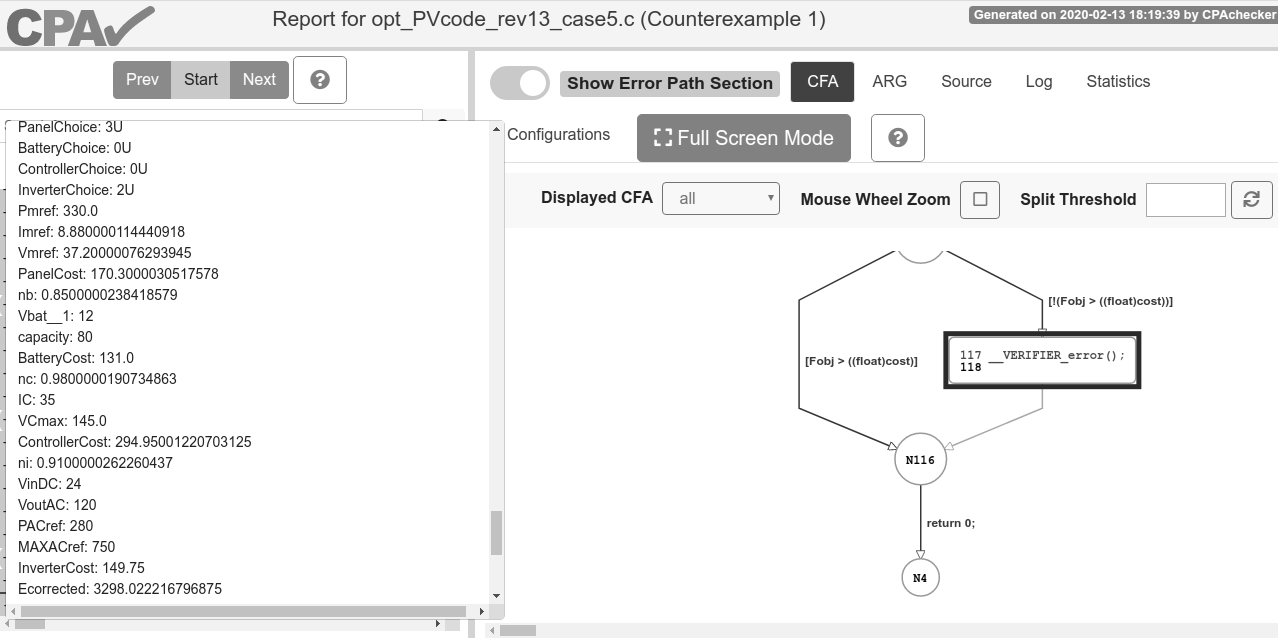
\includegraphics[width=0.9\textwidth]{CPA_opt_c5.png}}
\centering
\caption{Counterexample generated by CPAchecker after validation of case $5$.}
\label{fig:CPAoptc1}
\end{figure}

Here we used ESBMC in incremental BMC configuration with Boolector; ESBMC was able to reach the optimal sizing of case studies $1$, $3$, $4$, $5$, and $6$ with a FAIL/ SAT response, varying from $36$ minutes to $10$ hours. ESBMC, with this configuration, was unable to obtain an optimal solution in cases $2$ and $7$. Case $2$ produced a \textit{time out}. Moreover, case $7$ resulted in a UNSAT result, i.e., the verifier engine was unable to provide a feasible solution. However, this is not a bug, and it means that the available list of equipment can not produce a feasible solution that satisfies electrical compatibility or design requirements. This UNSAT situation was reached in less than one minute. These experimental results answer the \textit{EG2}.

HOMER Pro was able to evaluate six case studies (cases $1$, $2$, $4$, $5$, $6$, and $7$) under $30$ seconds; it was much faster than the proposed automated synthesis tool (cf.~\textit{EG3}). Case study $3$ could not be simulated since HOMER Pro does not have the battery autonomy adjustment feature, i.e., the tool always tries to feed the given load with electricity $365$ days/year. 

Some HOMER Pro drawbacks were also noted: (1) System equipment does not include an explicit charge controller. HOMER Pro includes a controller automatically to simulate the charge/discharge of batteries and to meet the load requirement. However, without costs or even with electrical characteristics such as maximum current and voltage, which are common during PV sizing. (2) HOMER Pro requires the inclusion of some battery specification to initiate optimization; however, it does not change the electrical specifications during simulation; the results presented are multiples of the original battery type suggested by the user. For example, it was started with a $83.4$ Ah lead-acid battery, and during simulation, HOMER Pro did not try to use other capacities or types. (3) HOMER Pro does not present the optimal solution in terms of connections of PV panel arrays, just the total in terms of power, i.e., it presents neither the models and the power of each PV panel nor the total of panels in series or parallel.

The authors had four PV systems deployed and monitored since June $2018$ in a riverside community in the State of Amazonas, Brazil, with demands of case studies $1$, $4$, $5$, and $6$, always with a $3$ $\times$ $325$ W ($3$S, a total of $975$ W) panels and $4$ $\times$ $220$ Ah ($2$S-$2$P $= 440$ Ah) lead-acid batteries.

%%%%%%%%%%%%%%%%%%%%%%%%%%%%%%%%%%%%%%%%%%%%%%%%%%%%%%%%%%%%%%%%%%%%
\subsection{Comparison Between Formal Synthesis and HOMER Pro, using PVsyst}
%%%%%%%%%%%%%%%%%%%%%%%%%%%%%%%%%%%%%%%%%%%%%%%%%%%%%%%%%%%%%%%%%%%%

If we compare the results of the formal synthesis with CPAchecker and ESBMC against those of HOMER Pro, we observed some distinct results in terms of the technical solution and cost (cf. Table~\ref{tab1}). Concerning the performance, there exists a vast difference in favor of HOMER Pro that obtained the results in considerably less time: few seconds in the opposite of an average of $4$ hours for the automated synthesis technique.
%
Particularly in the case of LCC, the cost varied from $11$\% to $44$\%, producing a higher estimation from the automated synthesis technique. However, considering that the cost of individual items of each database used to compose the optimal design is not the same among the tools, it is plausible to obtain distinct results.

On the one hand, concerning the PV panels sizing, the results presented by the automated synthesis were smaller in terms of power than the ones produced by the simulation tool. The difference varied from $19$\% to $65$\%. On the other hand, concerning the battery bank, the results were smaller in terms of capacity to the HOMER Pro. The difference was between $34$\% to $68$\%. The mathematical models are different and particular parameters can be tuned for each technique, and that can justify the difference, which was presented in all the case studies.

Those discrepancies are not easy to address without some real systems validation. However, we use the simulation software PVsyst to validate the optimal sizing produced, as shown in ~\ref{tab2}. Note that PVsyst has a pre-sizing feature, indicated in the table, that presents a minimum recommended sizing of PV panels and batteries (only), but without using manufacturers' data or models for it. This feature was used as reference mainly with HOMER Pro, where there is not equipment brands or models (only power and capacities specification). PVsyst was used with the field-deployed and the formal synthesis sizing solutions, where brands and models were simulated in PVsyst according to the sized system.

\begin{table}
\caption{Optimal sizing validation with PVsyst.}
\label{tab2}
\begin{scriptsize}
\begin{tabular}{c|c|c|c|c}
\hline
\hline
CS & \makecell{PVsyst\\(pre-sizing)}& \makecell{Field\\deployed\\validation}& \makecell{Formal synthesis\\sizing\\validation}& \makecell{HOMER Pro\\sizing\\validation}\\
\hline
\hline
CS 1 & \makecell{P= 1,166 W\\B= 381 Ah\\(minimum)} & \makecell{Not correct sizing \\Avail. $<$ 95\%\\(91.06\%)} & \makecell{No error found \\100\% of avail.} & \makecell{No error found\\Panels oversized in 2.16 $\times$\\Batteries oversized in 1.39 $\times$}\\
\hline
CS 2 & \makecell{P= 1,482 W\\B= 478 Ah\\(minimum)} & \makecell{NA\\There is not real PV system\\available for comparison} & \makecell{NA \\(TO result\\in Table~\ref{tab1})} & \makecell{No error found\\Panels oversized in 2.6 $\times$\\Batteries oversized in 1.74 $\times$}\\
\hline
CS 3 & \makecell{Not possible to \\simulate\\(autonomy $<$ 24h)} & \makecell{NA\\There is not real PV system\\available for comparison} & \makecell{Only technique that\\produced solution} & \makecell{NA\\(autonomy $<$ 24h)}\\
\hline
CS 4 & \makecell{P= 1,078 W\\B= 354 Ah\\(minimum)} & \makecell{No error found \\95.76\% of avail.} & \makecell{No error found \\97.37\% of avail.} & \makecell{No error found\\Panels oversized in 2.24 $\times$\\Batteries oversized in 1.41 $\times$}\\
\hline
CS 5 & \makecell{P= 823 W\\B= 268 Ah\\(minimum)} & \makecell{No error found \\100\% of avail.} & \makecell{No error found \\100\% of avail.} & \makecell{No error found\\Panels oversized in 1.93 $\times$\\Batteries oversized in 1.56 $\times$}\\
\hline
CS 6 & \makecell{P= 1,299 W\\B= 421 Ah\\(minimum)} & \makecell{Not correct sizing \\Avail. $<$ 95\%\\(85.65\%)} & \makecell{No error found \\100\% of avail.} & \makecell{No error found\\Panels oversized in 2.42 $\times$\\Batteries oversized in 1.38 $\times$}\\
\hline
CS 7 & \makecell{P= 4,263 W\\B= 1,384 Ah\\(minimum)} & \makecell{NA\\There is not real PV system\\available for comparison} & \makecell{NA \\(UNSAT result\\in Table~\ref{tab1})} & \makecell{No error found\\Panels oversized in 2.9 $\times$\\Batteries oversized in 1.99 $\times$}\\
\hline
\hline
\end{tabular}
\\Legend: CS = case study; NA = sizing not available for validation; B = batteries capacity; P = panels power; Avail.= Availability (expected of 95\% or greater as a design requirement).
\end{scriptsize}
\end{table}

Each simulation with PVsyst took $4$ seconds. We were unable to validate case study $3$ using PVsyst since the battery autonomy is less than 24 hours, and only the proposed synthesis technique can perform the optimal sizing (PVsyst and HOMER Pro are limited for a 24 h minimum autonomy). Case studies $2$ and $7$ had only HOMER Pro sizing validation, because there exists no deployed equivalent system in the field, and the synthesis technique did not present a solution due to time-out and internal failures in the underlying verification engine. %(our technique presented a \textit{time out} in case study $2$ and an \textit{UNSAT} in the case study $7$).

Overall, those comparisons among our approach, the optimization software, and the deployed systems, with validation through simulation tool, show that the synthesis solution is sound, which answers \textit{EG1 and EG3}.

HOMER Pro suggests a value in kW for the inverters that are very close to the maximum load of every case study, and it is just a reference value and not a commercial value of the inverter employed. The proposed synthesis tool, however, presents inverters that are commercial and can be bought off-the-shelf. Moreover, our synthesis approach considers surge power demand from the house, which is not considered by HOMER Pro or PVsyst. This feature is a definite advantage of the formal synthesis method.

HOMER Pro does not include charge controllers as a specific item of equipment in its mathematical model; only the synthesis tool presents a commercial controller and includes it during the cost analysis. The formal synthesis method, therefore, presents more reliable results than HOMER Pro.

In summary, our synthesis tool can present a solution that is far more detailed and closer to commercial conditions than the solution presented by HOMER Pro. In particular, the automated synthesis method can provide all the details of every component of a PV system solution, with complete electrical details from the manufacturer datasheet, including the model of the component, nominal current, and voltage. In this respect, even the name of the manufacturer can be cited (in Table~\ref{tab1}, it was removed to avoid unauthorized advertising). Moreover, the validation through PVsyst simulation, using the PV sizing produced by HOMER Pro and our synthesis approach, shows that our results are feasible and not as oversized as HOMER Pro results, mainly concerning PV panels.

%---------------------------------------------------------------------------
\subsection{Threats to validity} 
%---------------------------------------------------------------------------

We have reported a favorable assessment of the proposed method. Nevertheless, we have also identified four threats to the validity of our results that constitute future work. (1) improvement of the power reliability analysis: to include loss of load probability or loss of power supply probability, which can make the analysis more accurate. (2) improvement of the system cost analysis by including operational and maintenance costs to the adopted LCC analysis. (3) to increase the equipment and manufacturers database: this will increase the optimization complexity, but the result will also allow improved sizing. (4) the underlying symbolic verifiers employed here perform bit-precise verification based on the Floating-Point (FP) theory. We could use a real arithmetic strategy to tackle these equations; however, in this study, we have exploited the FP arithmetic, which is an approximation of the real one. 

%------------------------------------
\section{Conclusions} 
%------------------------------------

Our novelty relies on a practical approach to pursuit the optimal solution of PV systems using contemporary formal methods. The use of formal synthesis to design PV systems has no precedent in literature; we show that the results of our approach, using seven case studies, are promising. Our synthesis tool can present a solution, which is far detailed and closer to the commercial reality than the solution presented by HOMER Pro, a state-of-the-art commercial tool. In particular, the battery autonomy feature, together with the details of every component of a PV system solution, is an advantage for our synthesis approach. These technical details are essential for the owner of the PV system since the industry demands proximity between the result presented by off-the-shelf optimization tools and the items of equipment for solar systems available on the market to achieve accuracy. It is worth mentioning that our synthesis technique was developed and used open-source tools and environment, in contrast to the optimization and simulation tools used in this work. Lastly, the use of data from real deployed systems in Amazonas State (Brazil) and the validation through PVsyst was essential to validate the comparison.

%
% ---- Bibliography ----
% BibTeX users should specify bibliography style 'splncs04'.
% References will then be sorted and formatted in the correct style.
%
\bibliographystyle{splncs04}
\bibliography{trindadeThesis}
%
\end{document}
%\subsection{Design and Simulation of Solar PV systems}
%The design and validation of a PV system can be done by hand or with the aid of a software tool. In order to address different aspects of the PV system design, there are various software tools available in the literature~\cite{Rajanna,Rawat}.
%public domain and commercial software available for the PV market. 
%According to \cite{Brooks}, t
%%%%%%%%%%
%
%The capabilities of tools available in the literature range from simple solar resource and %energy production estimation, %to site survey and system design tools,
%to complex financial analysis and project optimization. At this study, the commercial simulation tool HOMER PRO was selected to be used at the case studies in order to be compared with the automated verification tools.
